
Alcune informazioni specifiche sono state allegate, approfondite da fonti esterne anche se non specificatamente spiegate all'interno dell'intervista, in modo da sottolineare tutte le procedure e i requisiti da conoscere per poter trattare la vendita alle pubbliche amministrazioni.

%------------------------------------------------
\subsubsection{Prima Intervista} % Sotto_Sotto-Sezione

\medskip

%Per le Interviste questo metodo è ottimo:
%\begin{description}[style=nextline]
%\item[DOMANDA]RISPOSTA  Fare attenzione alle lettere accentate che potrebbero non essere riconosciute
%non scordare di mettere la chiusura di description alla fine   \end{description}

\begin{description}[style=nextline]
    \item[Salve signor Rossi, innanzitutto potrebbe spiegarci esattamente di cosa si occupa la sua azienda]
    La nostra azienda offre servizi e vendita di prodotti sia a privati che a pubbliche amministrazioni. \newline
    La vendita riguarda apparecchiature elettroniche di uso comune legate specialmente all'informatica, dai personal computer ai suoi accessori, dai monitor a componentistica per la gestione di rete, mentre i servizi che offriamo comprendono prestazioni singole come per quanto riguarda ad esempio riparazioni e ripristino di computer, contratti di assistenza "on center", che significa letteralmente sul luogo, cioè contratti di durata solitamente tra i quattro mesi e l'anno, per i quali il cliente paga una quota prestabilita per ricevere assistenza in tempi relativamente brevi, e infine contratti a chiamata, che comprendono installazioni di apparecchiature elettroniche, come ad esempio di lavagne multimediali nelle scuole, che è un servizio offerto appunto a delle pubbliche amministrazioni.

    \item[Ci interessa particolarmente la vendita alle pubbliche amministrazioni, ci potrebbe spiegare nello specifico come funziona?]
    Per questioni burocratiche le pubbliche amministrazioni devono redigere delle gare pubbliche effettuando le cosiddette "richieste di offerta" sul mercato elettronico delle pubbliche amministrazioni chiamato MEPA.\newline
    Qui si trovano le richieste di offerta, l'azienda partecipa pubblicamente a queste gare, e poi in base all'esito della gara si pu\ò stipulare o meno il contratto.\newline
    C'è anche la possibilità per un istituto statale di fare una trattativa diretta con una particolare azienda abilitata sul MEPA senza la necessità di passare per una gara pubblica.

    \item[Quindi una volta che la vostra azienda partecipa ad una gara qual è l'iter effettivo di vendita e spedizione?]
    Per poter partecipare alla gara si accettano tutte le richieste fatte nello specifico sia che riguardino i prodotti o questioni di carattere legale come ad esempio la garanzia. Quello che manca a questo punto è proprio fare un ordine del prodotto dal fornitore per poi spedirlo oppure erogare direttamente il servizio richiesto. Nel caso di servizio esso viene erogato immediatamente mentre per un ordine i tempi di attesa sono quelli di spedizione del prodotto da parte del fornitore. La vittoria della gara di per se consiste nella firma del contratto.

	\item[Perciò la vendita ad una pubblica amministrazione come si differenzia da una vendita ai privati?]
	Ovviamente la differenza sta nelle modalità con cui le pubbliche amministrazioni acquistano un prodotto, infatti non è il cliente ad andare dal venditore, ma potremmo dire che sono i fornitori che vanno dal cliente. In più da parte del venditore ci deve essere la possibilità, nonchè la volontà, di rispondere ad una gara nei termini da essa richiesti.\newline
	Nella realtà c'è poi il problema della limitatezza della disponibilità dei prodotti richiesti, in quanto il fornitore può non avere la disponibilità necessaria per rispondere alla richiesta della gara.
	In particolare nelle trattative dirette dove la richiesta è diretta. In questo caso sta a noi rivolgerci ai fornitori per poter trovare una soluzione in modo da accettare la richiesta.
	In alcuni bandi ad esempio viene richiesto specificatamente un prodotto con il suo codice prodotto, bisogna quindi rispondere ad una richiesta molto specifica, in altri casi viene chiesto un prodotto con certe caratteristiche.

	\item[Ed il fatto che sia il venditore che debba adattarsi a quella che è la richiesta del cliente quali ripercussioni ha sul business? Le pubbliche amministrazioni hanno delle specie di convenzioni?]
	Non sono le pubbliche amministrazioni ad avere delle convenzioni con i venditori bensì sono i bandi ad avere un tetto massimo di spesa. Collegandosi al come questo impatta sull'azienda, ciò implica che talvolta si abbassino i propri margini di guadagno per aggiudicarsi una gara.\newline
	Non esiste il concetto di convenzione, i prezzi sono imposti dal mercato in quanto spesso il metodo di giudizio per aggiudicarsi una gara è proprio chi fa il prezzo minore.\newline
	Noi nei cataloghi abbiamo il prezzo di vendita del fornitore, il margine di guadagno viene deciso a posteriori durante la partecipazione alla gara.
	Di solito si tiene una quota percentuale fissa guadagno del 10\% però se con questa percentuale si sfora il tetto massimo può avere senso abbassare la quota per entrare nella gara e vincere.\newline
	Questa tipo di operazione ha senso su vendite più grosse, in quanto il guadagno è inferiore ma su volumi maggiori. Per un computer da 300 euro invece, il 10\% è 30, se 10\% è troppo non lo vendo, non conviene venderlo a meno.


	\item[A proposito di cataloghi, con i fornitori quali rapporti ci sono?]
	La realtà del rapporto con i fornitori è che quando effettuiamo un acquisto, noi paghiamo le spese di spedizione, quindi con i fornitori non c'è un accordo fisso, e quindi il costo delle spedizioni deve essere considerato durante la partecipazione ad una gara, ed è uno dei costi peggiori da tenere in considerazione, ma va calcolato con delle tabelle che può fornire il fornitore in base a vari fattori.
	Noi comunque per semplicità e per evitare di incadere in disagi di questo tipo non vendiamo alle isole, soprattutto per questi costi maggiorati di spedizione.

	\item[Perciò questi cataloghi da cui voi scegliete i prodotti da vendere li fornisce il fornitore?]
	Sì, esatto. I prodotti che noi vendiamo sono quelli che hanno i fornitori, quindi il nostro modello di business è il dropshipping, signfica non abbiamo un magazzino, se la richiesta non può essere soddisfatta dal fornitore rispondiamo di no, specie per le richieste dirette, altrimenti non partecipiamo proprio alla gara.\newline
	Non c'è per forza un rapporto diretto con il fornitore. Per le richieste generiche abbiamo dei cataloghi, quindi non viene sempre contattato, ci basiamo su quello come database, che viene aggiornato una volta al mese, è in formato digitale, fondamentalmente ci viene fornita una nuova tabella excel mensilmente.

	\item[Molto bene, voi offrite servizi oltre che prodotti. Nelle gare essi in che forma vengono descritti e come vengono valutati?]
	Le richieste di servizi sono molto generiche, i servizi sono richiesti con una descrizione generica della prestazione. Da parte nostra bisogna stimare il loro costo, il che non è una cosa banale.\newline Solitamente non si lavora ad ore ma si lavora per tipo di lavoro svolto, quindi è difficile standardizzare il costo della prestazione. Può essere semplice definire un costo per certi servizi, come ad esempio la formattazione di un computer, che richiede generalmente un tempo standard di lavorazione, ma risulta molto più difficile rispondere alla richiesta di installazione di una rete wifi, per cui il tempo di lavoro varia in base alla dimensione, alla struttura ed altri fattori.\newline Sarebbe molto interessante trovare un sistema per standardizzare in qualche modo questo processo.


	\item[Le abilit\`{a} del personaggio, in pratica, cosa sono?]Le abilit\`{a} sono delle mosse speciali che vanno ad incrementare il valore di una o pi\`{u} statistiche del personaggio. Per farti un esempio, l'abilit\`{a} Colpo Letale del guerriero va ad aumentare l'attacco del personaggio di un certo valore; mentre Elusivit\`{a} dell'arciere incrementa l'agilit\`{a} e la difesa

	\item[Ti ringrazio per la disponibilit\`{a} e la completezza]Figurati!Questa è una descrizione di come vanno pi\`{u} o meno le cose nel nostro come in molti altri Mmorpg, il Lead Programmer potrebbe esserti utile se ne vuoi sapere di pi\`{u}.

	%\item[]

    \end{description}


\newpage
%------------------------------------------------

\subsubsection{Seconda Intervista Lead - Programmer}
\medskip

\begin{description}[style=nextline]
    \item[Ciao sappiamo che siete al lavoro sul lato software del gioco, il nostro interesse \'{e} rivolto ai dati e vorremmo farti alcune domande]Chiedi pure.

	\item[Prima potresti descriverci in poche parole il software che state sviluppando?]Il nostro software \'{e} costituito da due parti. Il lato client che contiene tutto ci\`{o} che riguarda la gestione locale del gioco:caratteristiche mondo di gioco, modelli poligonali di personaggi e NPC, interfaccia grafica del giocatore. La parte server che si occupa dello scambio di informazioni con il client di gioco. Quindi tutto ci\`{o} che riguarda il combattimento, la compravendita di oggetti e le interazioni tra i giocatori ad esempio la chat di gioco.

	\item[Mi chiedevo se dati come le statistiche di base, l'esperienza ed il livello dei personaggi venissero aggiornati dall'applicazione quando per esempio si consuma qualcosa]Se intendi che lo fa il software si, prima lo faceva l'applicazione sul PC ma questo ci esponeva alle Cheat ora lo fa sempre il software ma sul server.

	\item[Ci faresti una breve descrizione dell'interfaccia grafica?] L'interfaccia grafica \'{e} composta, ai margini dal  ritratto del personaggio con il livello, la barra dei punti vita e punti mana. C'\'{e} una mini-mappa e le icone delle abilit\'{a} , sopra di loro troviamo la barra dell'esperienza. Ci sono pulsanti per accedere alla schermata dell'equipaggiamento, la schermata delle missioni e quella relativa all'inventario. Nella prima troviamo tutti gli oggetti indossati dal personaggio; al centro c'\'{e} anche un riepilogo delle statistiche del personaggio. Nella seconda troviamo un riassunto di tutti gli incarichi intrapresi e completati dal personaggio. Infine nello zaino possiamo visualizzare tutti gli oggetti immagazzinati e non utilizzati

	\item[Hai detto che il server si occupa della fase di combattimento, precisamente cosa fa?] Il combattimento consiste in una serie di calcoli che viene svolta dal nostro software sul server. Tuttavia il programma ha bisogno di alcuni dati per svolgere i conti, come le statistiche del personaggio e dell'attaccante, sia esso un altro giocatore o un NPC. Le statistiche del personaggio vengono ricavate dall'equipaggiamento che questo indossa,dalle abilit\`{a} utilizzate e da eventuali pozioni utilizzate. Una volta raccolte tutte queste informazioni il software fa la differenza tra l'attacco dell'attaccante e la difesa del suo obiettivo, il risultato viene tolto ai punti vita di quest'ultimo. E far\`{a} la stessa cosa per l'obiettivo contro l'attaccante

	\item[Il Director ci ha gi\`{a} dato un accenno alle statistiche di base del personaggio, ovvero forza intelligenza e destrezza. Ci chiedevamo se esistesse anche un attacco base nel caso il personaggio non possieda nessun arma.] Si, esiste un attacco base che in sostanza corrisponde all'attacco a mani nude del personaggio. Quando si trova senza armi per\`{o}, il personaggio non pu\`{o} utilizzare abilit\`{a}.

	\item[Ma l'equipaggiamento e le pozioni quali statistiche vanno a influenzare?]Quando parliamo di equipaggiamento parliamo di armi e armature. Le armi vanno ad aumentare l'attacco, possono anche modificare forza,intelligenza e destrezza. Le armature incrementano la difesa e, come le armi, possono modificare forza,intelligenza e destrezza. Mentre le pozioni influenzano una o pi\`{u} statistiche del personaggio, quindi potenzialmente tutte.

	\item[Ci chiedevamo se fosse necessario salvare la posizione dei personaggi e gli NPC?]Si,\'{e} molto importante. In questa maniera quando l'utente effettua il logout oppure il server va in crash, al successivo login potr\`{a} ricominciare dove si trovava. Mentre gli NPC ripartiranno da posizione iniziale che decidiamo noi; che comunque sia deve essere memorizzata

	\item[Ci puoi spiegare come vengono trattate le missioni dal lato software?]Il software si limita a contare gli oggetti missione raccolti dal giocatore o i mostri uccisi. Inoltre manda un messaggio a schermo quando la missione viene completata. Anche qui risulta importante salvare il progresso e il completamento delle missioni per lo stesso discorso delle posizioni.

	\item[Le missioni possono avere pi\`{u} obiettivi?]Si. Possono chiedere di uccidere diverse variet\`{a} di mostri oppure di raccogliere svariati oggetti.

	\item[Quali oggetti posso trovare nel bottino di un NPC ostile?]Puoi trovare equipaggiamento,pozioni e anche oggetti missione se il mostro \'{e} un obiettivo di una missione.

	\item[Posso avere oggetti uguali nel mio inventario?]Certo che si. Quando si trova un oggetto che si possiede gi\`{a} questi verranno accumulati

	\item[Gli NPC e gli oggetti hanno un livello?]Si lo hanno. Il livello degli NPC serve a far capire al giocatore se l'avversario \'{e} troppo forte o pure no. Mentre il livello negli oggetti viene inserito per un problema di bilanciamento. L'utilizzo di un oggetto molto forte a livelli basi andrebbe ad rovinare l'esperienza di gioco dell'utente

	\item[Parlando con il game director abbiamo capito che gli NPC amichevoli possono assegnare incarichi,vendere oggetti o insegnare abilit\`{a}. Possono svolgere pi\`{u} di una funzione alla volta?]Si,certo.

	\item[Se acquisto un oggetto da un NPC, poi lo rivendo allo stesso prezzo?]No, lo rivenderai ad un prezzo inferiore. Ogni oggetto avrà  il suo prezzo di acquisto e di vendita

	\item[Rimanendo nel settore della compravendita. \'{E} necessario tenere conto delle varie transazioni tra Giocatore-NPC e Giocatore-Giocatore?]Si, perch\'{e} offriamo al giocatore la possibilit\`{a} di annullare una transazione con un NPC. \'{E} possibile annullare uno scambio con un giocatore solo se vi è stata una truffa. In quel caso sar\`{a} un moderatore del gioco che si occuperà  della cosa quindi pu\`{o} far comodo sapere quando questa fosse avvenuta. Non è comunque necessario tenere traccia di tutte le transazione della vita di un personaggio, bastano quelle di una sessione di gioco.

	\item[Ci sono delle operazioni che dovete compiere periodicamente sul database?] Certo, ogni mese rilasciamo delle patch correttive per bilanciare le meccaniche di gioco. Quindi andiamo a regolare le statistiche di oggetti,NPC e abilità.

    \end{description}

\newpage

\subsubsection{Terza Intervista - Site Manager}


Abbiamo intervistato il manager di un sito che fornisce l'accesso al proprio gioco di ruolo e gestisce i giocatori e i loro acquisti e per acquisire conoscenze in merito alle modalità di gestione della parte esterna al gioco

\begin{description}[style=nextline]
    \item[Ciao, qual è il tuo ruolo nell?amministrazione del gioco?]Io mi occupo principalmente del settore marketing e gestisco l?interfaccia dell?utente con questo settore, in pratica definisco il business plan del gioco e come i giocatori vi entrano in contatto e eventualmente spendono soldi

	\item[Sappiamo che ci sono diversi modi di gestire un  gioco online, qual è il vostro piano?]Abbiamo scelto un piano ?pay to play?, ovvero gli utenti devono pagare una quota mensile per avere accesso ai server di gioco. Inoltre l'utente è tenuto ad acquistare la copia fisica o digitale del gioco e le sue eventuali espansioni per poter iniziare a giocare. Al fine di aumentare gli introiti abbiamo pensato di introdurre un item shop che mette a disposizione dei giocatori dei pacchetti di oggetti(equipaggiamento,consumabili). Questi oggetti vanno ad influenzare solamente l'estetica del personaggio, quindi non è possibile acquisire vantaggi rispetto ad altri giocatori come nei ?free to play

	\item[Cosa sono le espansioni?]Le espansioni sono delle aggiunte al gioco di base che possono essere nuove missioni nuovi, nuove abilità, nuovi oggetti, nuovi NPC. Rilasciamo nuove espansioni ogni 3 anni per invogliare i nostri utenti a rimanere sul gioco

	\item[Cosa puoi dirci invece della parte di gestione del sito?]Il sito \'{e} il primo luogo dove l'utente si reca per acquisire informazioni riguardanti il gioco ed eventualmente iscriversi. Una volta iscritto pu\`{o} collegarsi al nostro store online dove acquista i nostri prodotti. Tutto ci\'{o} comporta il tenere traccia di ogni giocatore, con i suoi dati utente, di fatturazione e delle sue carte di credito, nonch\'{e} dei suoi acquisti che, come nel caso della sottoscrizione possono avere una scadenza. E' necessario tenere traccia delle transazioni con gli utenti per calcolare le entrate con cui paghiamo il mantenimento dei server, che paghiamo mensilmente, nonch\'{e} i nostri stipendi.


	\item[E come gestisci questa mole di dati?]Abbiamo una base di dati che poi è la stessa a cui si appoggia il gioco, le nostre operazioni tuttavia sono  simili a quelle di un e-commerce, l?utente accede al sito e immette i suoi dati e fa i suoi acquisti, noi ci occupiamo di controllare questi dati immessi in caso di errori, aggiungiamo offerte e codici promozionali, revisioniamo i conti, il gioco si occupa dei pacchetti oggetto che un utente acquista che diventano di proprietà dei suoi giocatori.

\end{description}


%------------------------------------------------

%-------------------------------------------------------------------------
\subsubsection{Analisi delle Azioni e dei Processi Interni}

Partendo dalle interviste e integrando con la guida in linea di WOW le conoscenze sulle modalit\`{a} di gioco e sull'amministrazione dello stesso abbiamo costruito uno schema dei processi interni al gioco, separando ci\`{o} che avviene fuori dal gioco in verde, nell'amministrazione in arancione, ci\`{o} che accade nel gioco, oltre le semplici azioni \`{e} colorato a seconda dell'influenza sullo zaino in giallo o sull'equipaggiamento in blu.
Segue lo schema:


% \newpage
%
% \begin{landscape} %inizia un foglio landscape
%
%
% %include un file pdf che contiene lo schema ruotato e dimensionato correttamente
% 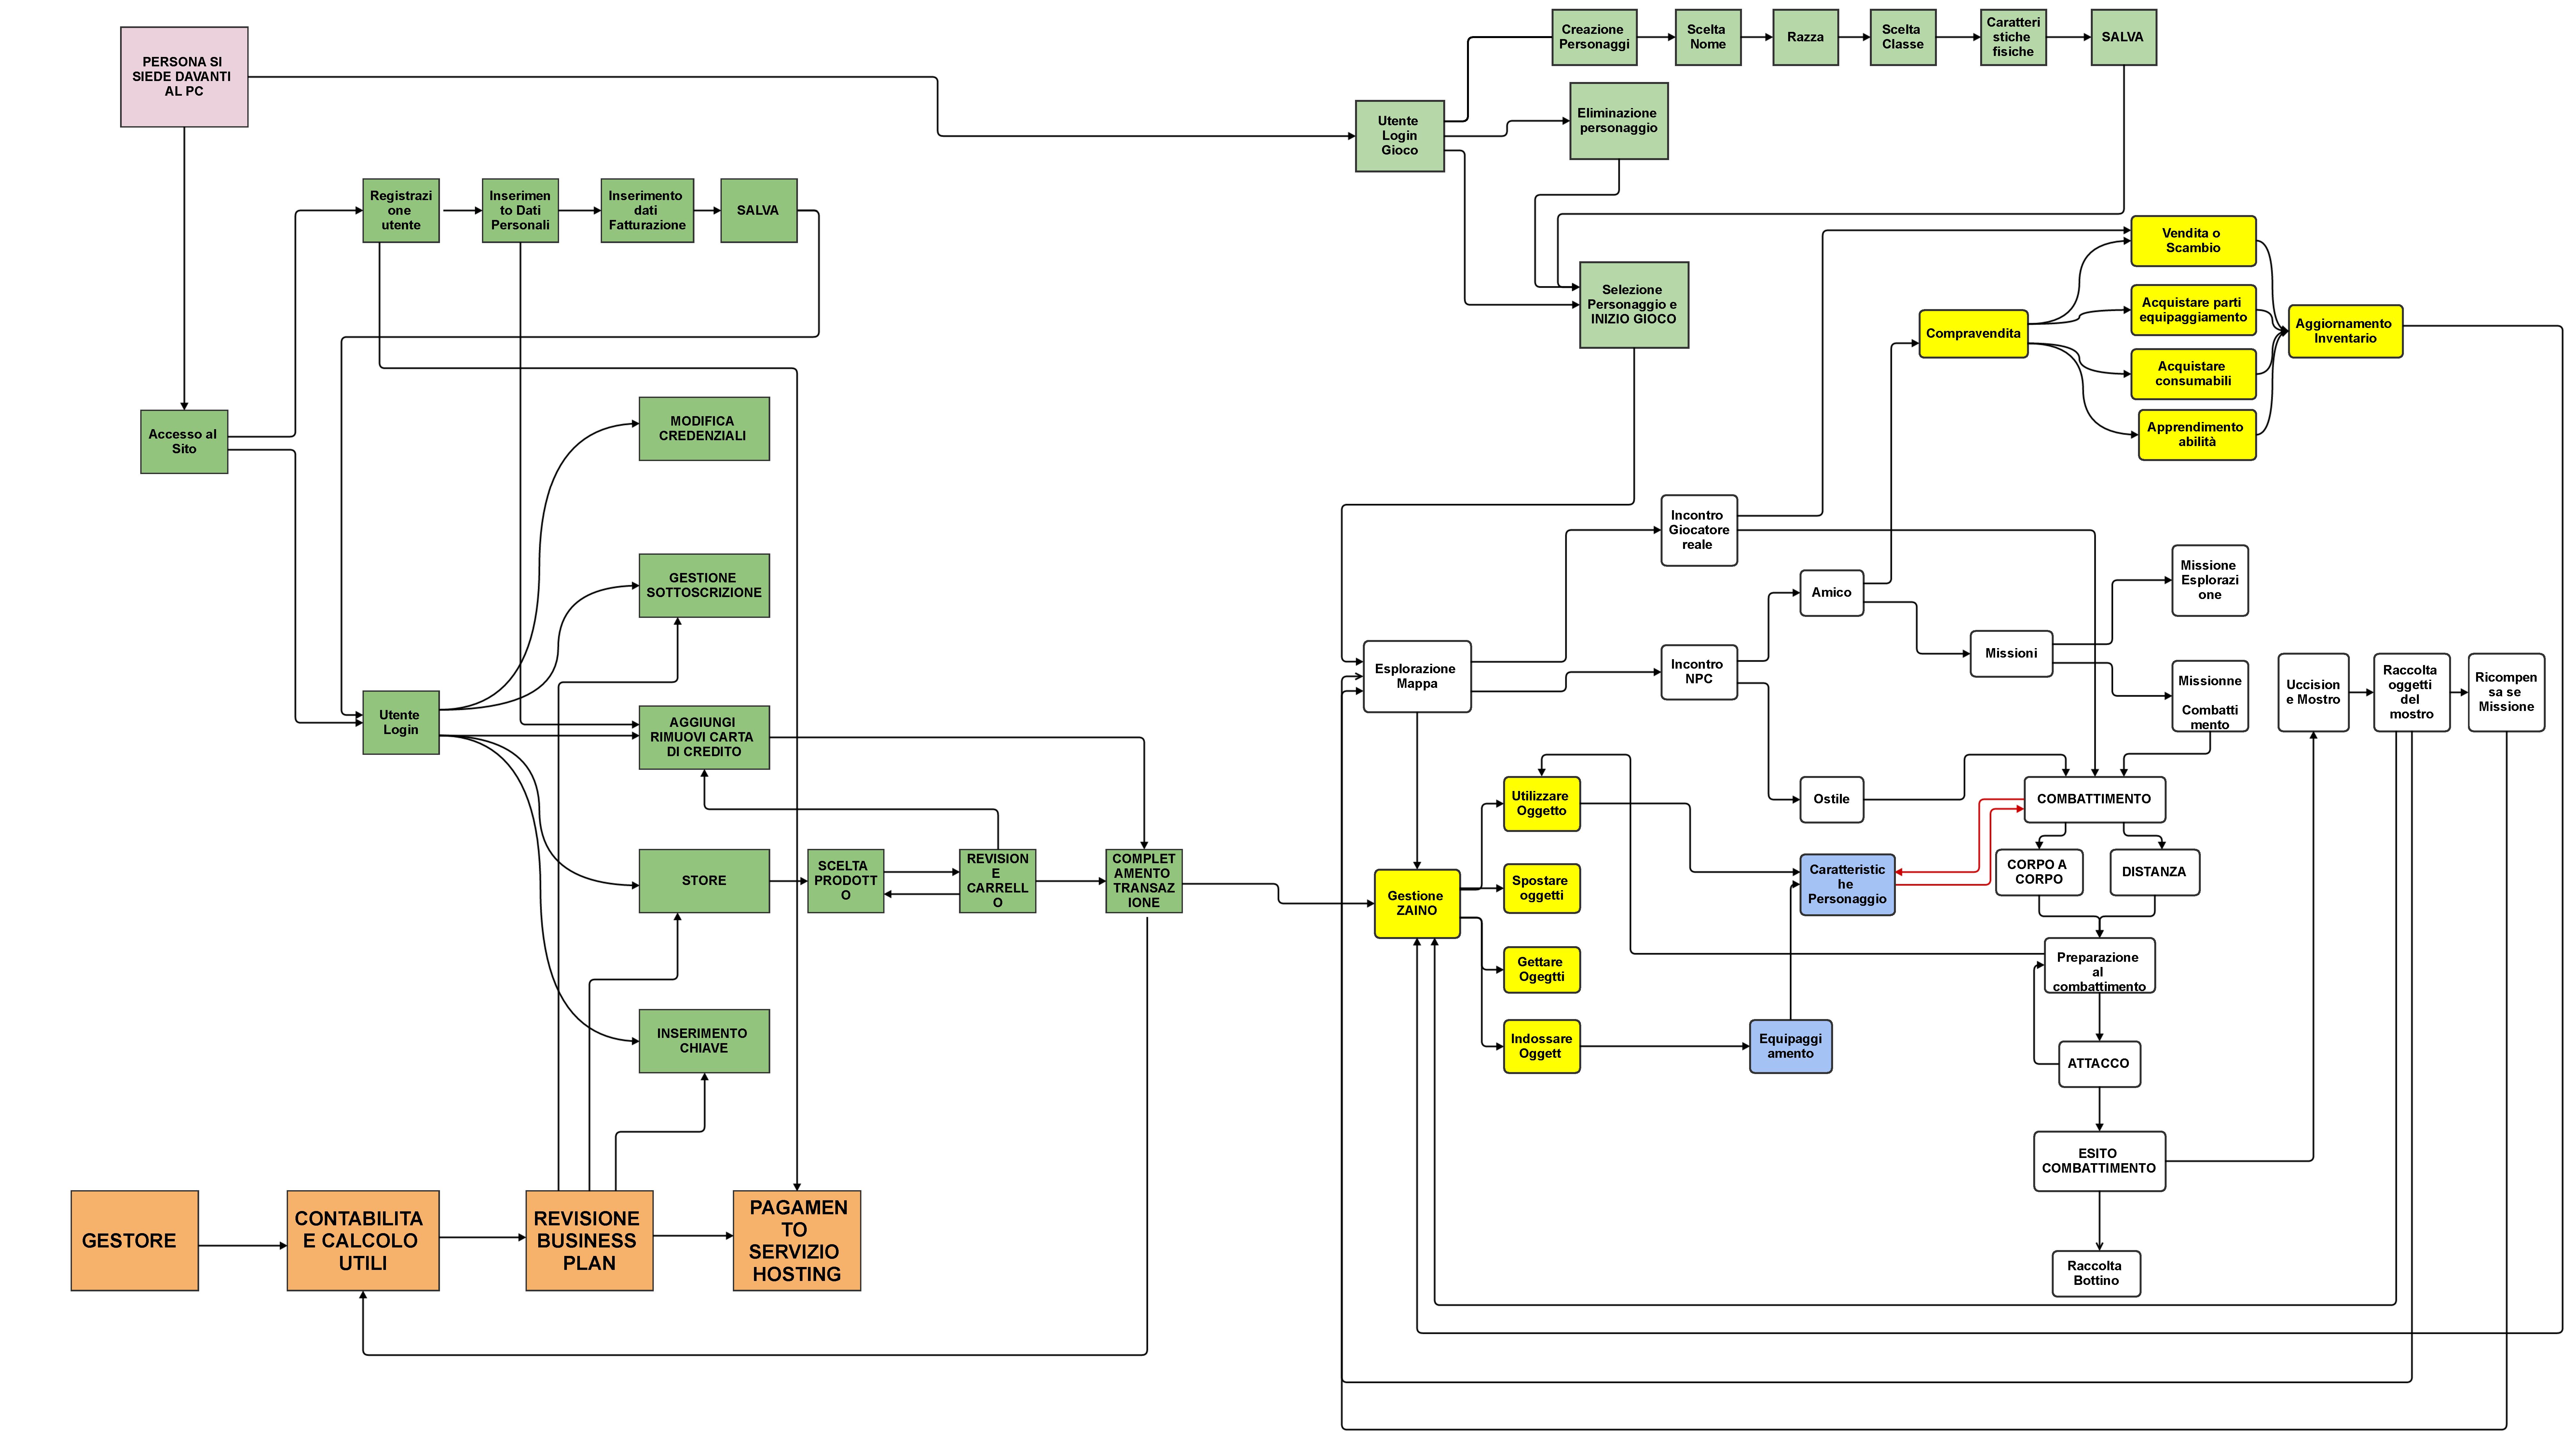
\includepdf[width=270mm, height=210mm, angle=90, keepaspectratio]{./pdf/sprocint.pdf}

\end{landscape}
